\documentclass[12pt]{article}
\usepackage{amsfonts, epsfig}
\usepackage[authoryear]{natbib}
\usepackage{array}
\usepackage{multirow}
\usepackage{graphicx}
\usepackage{fancyhdr}
\usepackage{amsmath}
\usepackage{amssymb}
\pagestyle{fancy}
\lfoot{\texttt{semtm0051.github.io} }
\lhead{Independent Component Analysis - Conor}
\rhead{\thepage}
\cfoot{}

\usepackage{tikz}
\usetikzlibrary{positioning}

\usepackage{ifthen}
\newboolean{nopics}
\setboolean{nopics}{true}


\begin{document}

\section*{Independent Component Analysis.} 

Principal Component Analysis is everywhere and it is easy to describe;
Independent Component Analysis (ICA) is often more useful but
difficult to explain, or, rather, the need for ICA is easy enough to
explain but the problem itself is a difficult one because there isn't
really a good, well defined, algorithm for finding the independent
components. Like PCA, it is useful to think a bit about it and to
learn a bit about what it does, but out treatment is going to be a bit
vague. The real message is to think about how things are represented,
how changing how data is encoded as a vector, or set of activations
over nodes, can disentangle its structure.

\begin{figure}[b]
  \centering
  \begin{minipage}[t]{0.48\textwidth}
    \centering
    \textbf{PCA}\\[2pt]
    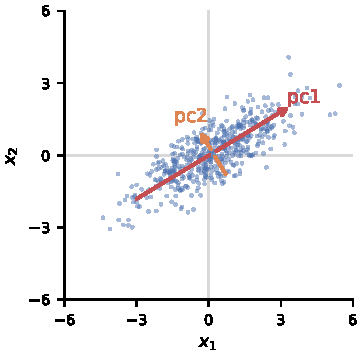
\includegraphics[width=\linewidth]{pca.pdf}
  \end{minipage}\hfill
  \begin{minipage}[t]{0.48\textwidth}
    \centering
    \textbf{ICA}\\[2pt]
    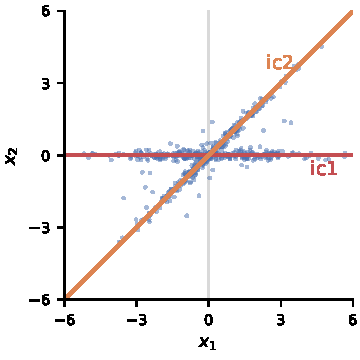
\includegraphics[width=\linewidth]{ica.pdf}
  \end{minipage}
  \caption{Left: PCA finds orthogonal axes ordered by variance. Right: ICA finds
    the (here non-orthogonal) directions along which the data are independent.}
  \label{fig:pca-ica}
\end{figure}


The motivation is straight forward and illustrated in
Fig.~\ref{fig:pca-ica}. It is common for the distribution of the data
suits PCA. This is what happens if the distribution is a multi-variate
Gaussian and for all sort of reasons this is a common distribution for
data; even when the data isn't precisely a multi-variate Gaussian, it
looks a bit like one. However, it isn't the only possibility. Imagine
looking at recipes for example and measuring how much ginger and
garlic they contain. If the recipe is Italian the amount of garlic
will vary but there will be hardly any ginger; for Indian recipes
there will be garlic and ginger and, in fact, they will be
proportional, the more garlic, the more ginger; indeed they will have
roughly the same amount by weight, so some dishes will have lots of
garlic and some little, but those same dishes will also have a lot of
ginger or a little. This is the situation we are cartooning in
Fig.~\ref{fig:pca-ica}ICA, the $x$-axis represents the amount of
garlic, the $y$-axis is the amount of ginger and the dots are
recipies, the two red lines pick out the two different cuisines.

This is often when ICA is useful, there is a choice, here, what sort
of cuisine, and then a continuous process whose details depends on the
discrete choice, here, the amount of ginger and garlic. In this case
the axes, horizontal for Italian food, along $x=y$ for Indian,
represent the \textsl{independent components} in recipe space.

\subsection*{fastICA}

I mentioned that we weren't going to look at how to do ICA in any
detail. There are basically two main algorithms, \textsl{infomax} and
\textsl{fastICA}. The infomax algorithm is extremely elegant, using
ideas from information theory in a tour-de-force of cunning
computation to produce a well-motivated approach to finding
independent component. However, fastICA is the more popular algorithm,
partly because it is fast, partly because the team who developed it
put a lot of effort into producing nice, optimized, robust,
implementations in lots of languages and finally, I think it helps
that the overall reason the algorithm works is less elegant that
infomax but easier to explain!

The idea behind fastICA is that mixtures of random processes tend to
be Gaussian. There is, in fact, a theorem called the \textsl{Central
  Limit Theorem} that tells us in a precise way that in precise
circumstances that there is a sense in which
\begin{equation}
  S = \sum_n \frac{X_1+X_2+\ldots+X_n}{n}
\end{equation}
tends towards a random variable with a Gaussian distribution as $n$
becomes large when the $X_i$ are independent identically distributed
random variables. The theorem gives means for `a sense in which',
`tends towards' and `becomes large'. However, the precise details of
the Central Limit Theorem doesn't concern us, what is important is a
vague lesson we can learn from it: adding random things up usually
gives us something that is more like a Gaussing than the things
themselves.

Carrying on with our recipe analogy wouldn't be impossible but it
might be a bit confusing! Lets consider a more classic example of when
ICA is useful and, in fact, one of the main places it is used. This is
the \textsl{cocktail party problem}. Imagine you are listening in to
two people, you and these people might be at a cocktail party, this
sounds unlikley in real life, do people still have cocktail parties,
but this is just a story. The two people are in different positions
and so sound of their voices is combined when it enters your ear as
some linear combination of each, the linear weights depend on how far
from your ear they are. Each voice changes amplitude independently,
the ear hears a combination of the two. In the way this story is told,
you actually have access to two different linear combinations, one for
each ear. So, there are two independent sources, each of the two
people and you have access to two different linear combinations, one
for each ear. The job of ICA is to allow you to seperate the two
combined signals into two different signals, one for each speaker.

This is completely unrealistic, we are very good at solving the
cocktail party problem but we don't solve it by relying on the small
different in amplitude in the signals entering each ear, we use a
whole set of techniques and it probably helps that our ears are such
an odd shape, but this is just a story and, as mentioned there are
version of the cocktail party problem where we do have a set of
observed signals corresponding to different weighted sums and where we
do use fastICA.

So, lets imagine we are in two dimensions and there are two random
variable, $X_1$ and $X_2$. These are independent, potentially
different processes, the two voices in our example, and for this to
work they aren't Gaussian. Now lets mix them:
\begin{equation}
  \left(\begin{array}{c}Y_1\\Y_2\end{array}\right)=M \left(\begin{array}{c}X_1\\X_2\end{array}\right)
\end{equation}
where $Y_1$ and $Y_2$ are the values we actually observe, the sounds
in our two ears, and $M$ is a mixing matrix, a $2\times 2$
matrix. This means $Y_1=w_{11}X_1+w_{12}X_2$ and
$Y_2=w_{21}X_1+w_{22}X_2$. Thus, the things we observe are more
Gaussian than the original variables. The idea is to find an unmixing
matrix $W$ so
\begin{equation}
  \left(\begin{array}{c}Z_1\\Z_2\end{array}\right)=W \left(\begin{array}{c}Y_1\\Y_2\end{array}\right)=WM\left(\begin{array}{c}X_1\\X_2\end{array}\right)
\end{equation}
Now if $W=M^{-1}$ then $Z_i=X_i$ and we will have found the original
unmixed variables.  Now the clever thing is that the closer $W$ is to
being the $M^{-1}$ the less Gaussian we might expect $Z_1$ and $Z_2$
to be, the closer each is to being just one of the $X_i$ the less it
is a mixture. The idea behind fastICA is to measure how Gaussian the
$Z_i$ are and then vary the coefficients of $W$ to minimize whatever
measure of ``Gaussian-ness'' is being used.


\subsection*{A language example}

We are going to look at a slightly complicated example, but I think a
fun one. It is complicated because it introduces another technology
called \textsl{word2vec}. The purpose word2vec is to map words to
vectors. The original ``skipgram'' word2vec approach was surprising
when it was introduced, it arrived soon after AlexNet and was part of
the revival of interest in neural networks. It is very different to
AlexNet though since it used a surprisingly shallow.

The idea is simple: take a big list of all the words in your
dictionary, a 10,000 vector for example, remember this was 15 years
ago. Give entries in this vector all the value zero. Now pick a word
in a text and turn the corresponding entry in your vector to one. Now
map your big vector to a smaller continuous vector, say
300-dimensional which we will call the latent space with the
activation pattern of that vector for your word just some vector in
the latent space $\mathbf{v}[$word$]$ and then map that vector to
another big vector corresponding to all words. This involves two big
matrixes $10000\times300$ matrix mapping the input to the latent space
and $300\times 10000$ to map to the output. Finally map the output
vector values to probabilities and train the two big matrices on an
objective based on the idea that these probabilities tell us which
words are near in the text to input word. Near here could mean
``within eight-wrods either side'' or ``in the same sentence''. After
we've done all this the latent space vectors, the
$\mathbf{v}[$word$]$s, are the things we wanted, vectors representing
words.

The thing that makes this useful is that it appears to produce vectors
that represent aspects of word meaning. Again, this is less remarkable
now; we have other more sophisticated transformer based approaches for
representing the meanings of words and, indeed, this is one of the
things that is happening in the layers of the transformers used in
large language models. Here, we are just introducing it as an example
of how ICA can pull out the structure of data and it is being used as
an example precisely to familiarize you with the way representation
works, the way neural networks map things from one vector to another
in ways that represent and organize the properties of the things in
question. Anyway, in the case of word2vec the original papers showed off about a sort of ``Euclideanization'' of the words, relationships like:
\begin{equation}
  \mathbf{v}(\text{Mozart})+[\mathbf{v}(\text{scientist})-\mathbf{v}(\text{Einstein})]\approx\mathbf{v}(\text{violinist})
\end{equation}
These examples where often highly cherry-picked, but it was still cool
at the time!

We won't use skipgram. It comes with a nice explaination but better
approaches were found afterwards; instead we use a fairly standard set
call \textsl{GloVe}; GloVe actually finds similar vectors to skipgram,
100-dimensional in the version we use, we won't go into the
details. Suffice to say, GloVe maps words to vectors and the vectors
are easily downloaded from the internet. We are going to do ICA on
GloVe.

The idea is to take the GloVe vectors for the twenty thousand or so
most common words, leaving out the hundred very commonest ones, words
like `the' and `of', which turn up everywhere and so tell us very
little, and to treat each word's vector as a data point, exactly like
the recipes in Fig.~\ref{fig:pca-ica}, except that now there are 100
dimensions rather than two. We run fastICA on these points, asking for
100 components, so that each word gets a new set of coordinates, one
for each independent component. To see what a component is `about' we
just list the words with the largest values along it. If we do the
same thing with PCA the lists are a bit of a jumble: a few of the
principal components are coherent, but most mix unrelated things, so
one, for example, has Ingushetia, the Sensex stock index, the PKK and
landslides. The independent components are much cleaner, most of them
pick out a single category you would recognise, and if we plot the
words against two of them, as in Fig.~\ref{fig:ica-words}, we see the
same two-armed picture as the recipes, with food words along one axis,
music words along the other and almost nothing in between: most words
are mostly about one thing. Here are five of the components, with the
words that score highest on each:
\begin{itemize}
\item \textbf{cooking:} teaspoon, tablespoons, sauce, garlic, chopped,
  onion, butter
\item \textbf{music:} albums, vocals, songs, band, guitar, jazz
\item \textbf{stock markets:} Topix, DAX, KOSPI, FTSE, Nikkei, Nasdaq
\item \textbf{computing:} desktop, Macintosh, Android, USB, software,
  server
\item \textbf{injuries:} spinal, ligament, knee, ankle, tendon,
  fracture
\end{itemize}
Not all the components are topics like these, some are about grammar
or style rather than subject matter, there is one, for example, made
up of intensifiers, incredibly, utterly, extremely, enormously, and
another of verbs ending in `-ing'; and a few are junk. Nonetheless, it
is striking that a method which knows nothing about language, which
only looks for directions along which the data is as un-Gaussian as
possible, pulls out so much of the structure of meaning.

\begin{figure}[t]
  \centering
  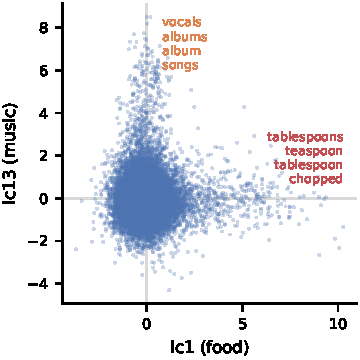
\includegraphics[width=0.48\textwidth]{ica_words.pdf}
  \caption{GloVe word vectors plotted against two of the independent
    components found by fastICA. Most words sit near the origin; words
    about cooking lie along the horizontal axis and words about music
    along the vertical one, with very few words scoring highly on
    both.}
  \label{fig:ica-words}
\end{figure}

\end{document}

